
% Due Date: 6/25/14

\chapter{Logical Dependence Analysis}
\label{chapter:logical}
The first stage in the Legion task pipeline
is logical dependence analysis. Given a stream
of sub-task launches from a common parent task, the 
dependence analysis stage is responsible for computing which 
tasks are {\em interfering} and therefore must have 
dependences (we give a formal definition of non-interference 
in Section~\ref{sec:noninterference}). Unlike other 
programming systems that compute dependences between 
tasks based on inferred data usage, either statically (e.g. 
by doing pointer analysis), or dynamically (e.g. transactional 
memory), Legion has specific names for the 
sets of data being accessed by tasks in the form 
of logical regions. The concrete names for different
sets of data provided by logical regions will
considerably simplify the dependence analysis.

A na\"{i}ve implementation of the Legion dependence 
analysis stage would perform a pairwise test for
non-interference between a sub-task and all of the
tasks launched before it in the same parent task.
For a stream of $N$ tasks, dependence analysis is 
known to require $O(N^2)$ non-interference tests
be performed\footnote{In Legion, non-interference
tests are actually performed between the regions
used by tasks. If tasks on average have $R$ region
requirements, then dependence analysis is actually
$O(N^2R^2)$.}. In practice, the size of $N$ is 
bounded by a sliding window reflecting tasks that
have yet to complete. A task only needs to perform
non-interference tests against tasks within this
window. Figure~\ref{fig:taskwindow} shows a 
representative example. Task $t_8$ only needs to
perform dependence tests against tasks in the
stream $S$ that remain within the window and 
therefore not complete. However, the 
task window is usually on the order of a few hundred 
to a thousand tasks in many applications. While 
finding an asymptotically superior algorithm for dependence 
analysis is unlikely, we can introduce data structures 
that can significantly improve the constant factors 
associated with the dependence analysis algorithm.

\begin{figure}[t]
\centering
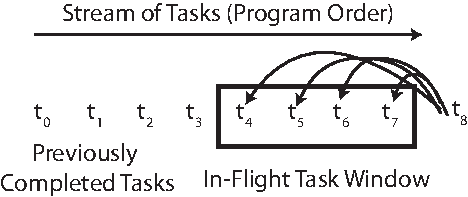
\includegraphics[scale=0.7]{figs/TaskWindow.pdf}
\caption{Example Task Window for Dependence Analysis\label{fig:taskwindow}}
\end{figure}

In this chapter, we begin by giving a precise 
definition of when two tasks are non-interfering 
(Section~\ref{sec:noninterference}). Based on
the properties of the non-interference test,
we design an algorithm that leverages the logical
region tree data structures maintained by the
runtime to accelerate non-interference tests 
(Section~\ref{sec:logtraversal}). We then 
elaborate on how storage for the meta-data
associated with dependence analysis is
efficiently maintained 
(Section~\ref{sec:logicaltree}). In
Section~\ref{sec:mapdepgraph}, we describe
the mapping dependence graph produced by
the logical dependence analysis.
Finally, we describe an optimization 
for memoizing the results of the dependence 
analysis in Section~\ref{sec:tracing}.

\section{Task Non-Interference}
\label{sec:noninterference}

Before proceeding with our discussion of how
we implement the dependence analysis stage, we 
first need to give a precise definition of
what it means for two tasks to be non-interfering.
Two tasks are non-interfering if all pairs of region
requirements between the two tasks are 
non-interfering.  A pair of region requirements
are non-interfering if any one of the following
three disjunction non-interference conditions
are met:

\begin{itemize}
\item {\bf Region Disjointness} - the logical
regions in the two region requirements are disjoint
(e.g. there are no shared rows).
\item {\bf Field Disjointness} - the sets of fields
requested by each of the two region requirements
are independent (i.e. there are no shared columns).
\item {\bf Privilege Non-Interference} - either
both region requirements are requesting read-only
privileges, or both region requirements are 
requesting reduction privileges with the same
reduction operator.
\end{itemize}

Figure~\ref{fig:noncases} gives a visual depiction
of the three different non-interference criteria 
from the node's logical region in the circuit 
simulation from Chapter~\ref{chapter:model}. 
The red and blue rectangles illustrate the data
requested from two different region requirements.
Non-interference can be proven in any of the three
dimensions: if the two logical regions access
disjoint sets of rows, if the sets of fields requested
are disjoint, or if the privileges are non-interfering.

\begin{figure}[h]
\centering
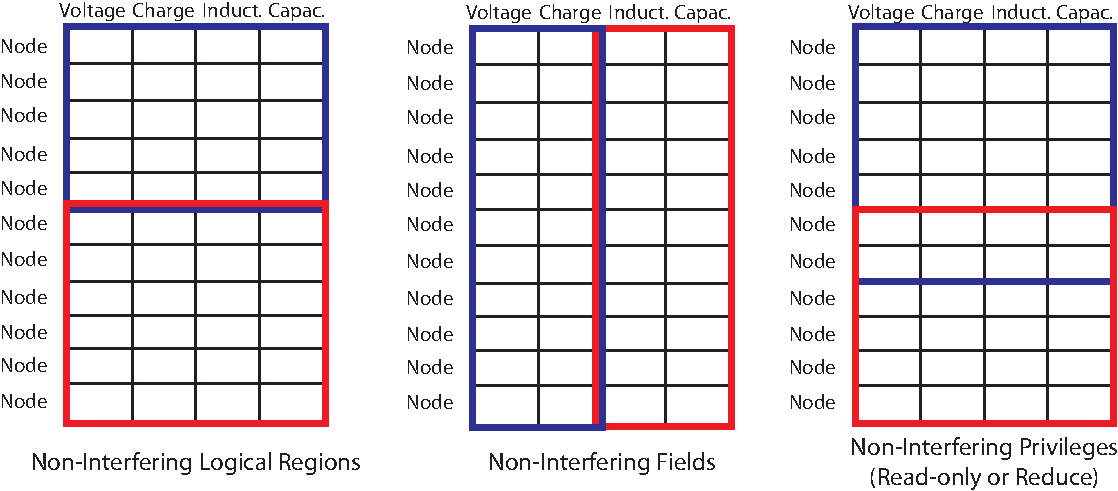
\includegraphics[scale=0.7]{figs/NonInterfering.pdf}
\caption{Example Non-Interference Criteria from the Circuit Simulation
\label{fig:noncases}}
\end{figure}

Due to the disjunctive nature of the three conditions,
they can be applied in any order.  If any of the
three non-interference criteria are met, then the 
pair of region requirements are non-interfering 
and testing the remaining conditions can be skipped. 
Consequently, the order in which these criteria are
tested can have a significant performance impact.
It is therefore important that we pick an order for
testing these conditions that minimizes the number
of non-interference criteria tested.

The ordering that we select is region disjointness,
field disjointness, and finally privilege 
non-interference.  This ordering stems from the 
observation that Legion programs commonly express 
data parallelism at several different granularities 
both across nodes and within nodes. It is therefore 
most likely that two tasks will be proven to be 
non-interfering using the disjointness of their 
logical regions. After this, field set disjointness 
is most likely.  Finally, privilege non-interference 
is a more complicated test and is therefore placed 
last where it is least likely to be performed.  
While it is possible to write Legion applications that
perform better with a different test ordering, it 
has been our experience that the performance of this 
ordering is sufficient for achieving high 
non-interference test throughput. As we show in 
Section~\ref{sec:logtraversal}, this ordering also
lends itself to a natural implementation based
on logical region trees.

\newcommand{\appnonint}[7]{
\begin{tikzpicture}[every node/.style={inner sep=0,outer sep=0}]
\node (n1) at (0,0) {\footnotesize\begin{tabular}{c}no tests \\ $0.0 \%$\end{tabular}};
\node (n2) at (2,1) [minimum width=0.4in] {\footnotesize\begin{tabular}{c}regions \\ $#1 \%$\end{tabular}};
\node (n3) at (2,0) [minimum width=0.4in] {\footnotesize\begin{tabular}{c}fields \\ $#2 \%$\end{tabular}};
\node (n4) at (2,-1) [minimum width=0.4in] {\footnotesize\begin{tabular}{c}privileges \\ $#3 \%$\end{tabular}};
\draw [->] (n1.north east) -- (n2.west);
\draw [->] (n1) -- (n3);
\draw [->] (n1.south east) -- (n4.west);
\node (n5) at (4.5,1) [minimum width=0.7in] {\footnotesize\begin{tabular}{c}regions+fields \\ $#4 \%$\end{tabular}};
\node (n6) at (4.5,0) [minimum width=0.7in] {\footnotesize\begin{tabular}{c}regions+privileges \\ $#5 \%$\end{tabular}};
\node (n7) at (4.5,-1) [minimum width=0.7in] {\footnotesize\begin{tabular}{c}fields+privileges \\ $#6 \%$\end{tabular}};
\draw [->] (n2) -- (n5);
\draw [->] (n2) -- (n6);
\draw [->] (n3) -- (n5);
\draw [->] (n3) -- (n7);
\draw [->] (n4) -- (n6);
\draw [->] (n4) -- (n7);
\node (n8) at (7,0) {\footnotesize\begin{tabular}{c}all tests \\ $#7 \%$\end{tabular}};
\draw [->] (n5.east) -- (n8.north west);
\draw [->] (n6) -- (n8);
\draw [->] (n7.east) -- (n8.south west);
\end{tikzpicture}
}

\begin{figure}
\centering
\begin{tabular}{c}
\subfloat[Circuit]{
\appnonint{69.0}{43.6}{25.7}{81.1}{76.3}{60.5}{85.5}
} \\
\subfloat[Fluid]{
\appnonint{99.2}{43.2}{20.5}{99.4}{99.7}{54.1}{99.8}
} \\
\subfloat[S3D]{
\appnonint{33.1}{98.4}{32.2}{98.6}{52.7}{99.4}{99.5}
} \\
\end{tabular}
\caption{Non-Interference Test Success Rates by Application\label{fig:nonint_venn}}
\end{figure}

To provide empirical evidence for our chosen ordering
of these tests, Figure~\ref{fig:nonint_venn} shows decision
diagrams for potential orderings of non-interference
tests for three real world applications: a circuit
simulation, a fluid flow simulation, and the combustion
simulation S3D discussed in Chapter~\ref{chapter:s3d}.
At each node of the decision diagrams, we show the
percentage of non-interference tests that would
succeed with that subset of tests. The percentage at
the end shows the overall percentage of non-interference
tests that succeed for a given application.

Ideally, we want to minimize the overall cost of the 
non-interference tests, which favors the early use 
of cheaper and/or more efficient tests. Although
there is considerable variability between applications,
region disjointness is the most effective test
overall. The use of region tree data structures
is essential to making this test inexpensive, and it
is the clear choice for the first test. Field disjointness
is the next obvious test as it finds significant
parallelism, especially in S3D. By using {\em field
masks} (discussed in Section~\ref{subsec:fieldmasks}) this 
test can also be made inexpensive which justifies 
performing it second. Finally, the more expensive 
privilege non-interference test is placed last to 
minimize the number of invocations.

\section{Logical Region Tree Traversal Algorithm}
\label{sec:logtraversal}

The goal of the logical region tree traversal algorithm
is to improve the efficiency of the dependence
analysis for a stream of sub-tasks $S$ within a
parent task $P$.  To perform the dependence 
analysis for any sub-task $T$ in $S$, we
need to find all other tasks that come before
$T$ in $S$ that interfere with at least one of
the region requirements requested by $T$. We therefore 
need to perform a separate analysis for each 
region requirement of $T$.

%We say that all the sub-tasks
%in $S$ are analyzed within the {\em context} of
%the parent task $P$.  A context denotes the subset
%of privileges that the parent task owns on the
%region tree as part of its execution. (A context
%will also be given a technical definition in
%Section~\ref{subsec:logicalctx}.) 

To detect interference on region requirements,
our analysis operates over the logical region 
tree forest. As part of our analysis, we ensure 
that after each task in $S$ has performed its
non-interference tests, it registers itself as a
{\em user} of the region tree node for each logical
region on which it requests privileges. A user 
record stores information about the task including
its requested fields, privileges, and coherence.
User records allow later tasks to determine whether
dependences should be registered from later tasks
in $S$. By registering users at the region tree 
nodes on which they requested privileges, we will
be able to easily elide non-interference tests based
on logical region disjointness (the first 
non-interference condition from 
Section~\ref{sec:noninterference}). In practice,
we do not need to store all the users on each logical
region tree node from previous tasks in the 
stream $S$. Instead, we can aggressively prune tasks 
that have finished executing or for which we can prove 
there exists transitive dependences.  We discuss these 
optimizations further in Section~\ref{sec:logicaltree}.

To perform the dependence analysis for a sub-task $T$,
we need to traverse the region tree forest for each region
requirement in $T$ to find any potential tasks from 
$S$ that are not disjoint on region usage. We first
compute the path from the logical region requested
to the corresponding logical region on which the 
parent task $P$ owns privileges. This path is 
guaranteed to exist because of the restriction 
enforced by the Legion programming model that 
all sub-tasks can only request privileges for 
a subset of the privileges held by the parent task 
(see Section~\ref{subsec:subtasks}). Using this
path we can immediately determine the nodes in the
logical region tree that must be visited because
they are interfering on region disjointness. This
set of nodes includes all nodes in the region tree
along the path, as well as any sub-trees of nodes
along that path that may contain interfering nodes.
By computing this path and any potential interfering
sub-trees, we immediately elide any region requirements
of previous tasks that are disjoint on region usage,
including region requirements in different region
trees within the region tree forest.

As an example of the region tree path, consider a 
sub-task launched inside of the {\tt simulate\_circuit}
task from the example in Chapter~\ref{chapter:model}.
Figure~\ref{fig:interferencepath} illustrates both the
computed path and other logical regions that would need
to be analyzed for interferences for a region requirement
requesting privileges on the {\tt r\_all\_shared} logical
region. The interference path would run from the root node
of the logical region tree where the {\tt simulate\_circuit}
task has privileges to the {\tt r\_all\_shared} logical region
where the task is requesting privileges. In addition, the task
would also need to visit all the sub-trees of the 
{\tt r\_all\_shared} logical region. All of the nodes that
would need to be analyzed for interference are colored in
red. Nodes that can be skipped due to being non-interfering
are shown in blue. It is important to note that the two-level
partitioning scheme that we chose in Chapter~\ref{chapter:model}
is what allows this analysis to directly omit all logical
regions in {\tt r\_all\_private} nodes from consideration
when analyzing region requirements that request privileges
on logical regions in the {\tt r\_all\_shared} logical region
sub-tree.

\begin{figure}[h]
\centering
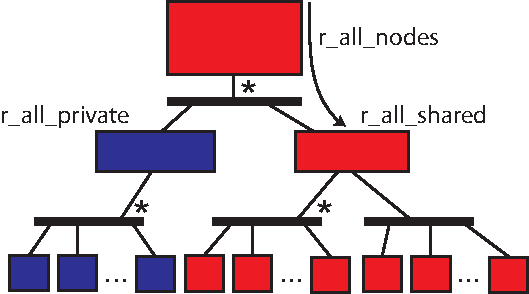
\includegraphics[scale=0.7]{figs/NonInterferencePath.pdf}
\caption{Example Non-Interference Path for Dependence Analysis
\label{fig:interferencepath}}
\end{figure}

Having determined the set of region tree nodes that
must be examined because they are interfering on 
logical region usage, we can now perform the second
dimension of the non-interference test based on
field usage. For each node that interferes based on
region usage, we iterate through the
list of users registered at the node.
We then check whether the set of fields requested
by each user is disjoint from the 
set of fields in the region requirement being
tested from $T$. If they are disjoint, then the
two region requirements are non-interfering, otherwise
we perform the non-interference test on privileges.
If both the field sets are interfering and the 
privileges are interfering, then we record a 
dependence between the two tasks, otherwise that
pair of region requirements is non-interfering.
Finally, after finishing the analysis for a
region requirement, we register the region 
requirement at the destination node of the
path, ensuring that any future sub-tasks in 
the stream $S$ will be able to determine
the necessary dependences.

While this discussion has primarily described 
sub-tasks as the elements within the stream $S$,
because the region tree analysis is performed
based on region requirements, the analysis is
easily generalized to all other operations within
the Legion programming model, including inline
mappings and explicit copy operations that also
use region requirements to describe their data usage.

\section{Logical Region Tree Data Structures}
\label{sec:logicaltree}
While the correctness of the traversal algorithm
described in the previous section is easy to
determine, achieving high-performance requires
optimization of both the algorithm as well as the data
structures used for the traversal. We first give 
a brief description of how region tree data structures 
are stored in the Legion runtime in 
Section~\ref{subsec:logicalshape} and then we describe 
each of the optimizations in subsequent sections.

\subsection{Region Tree Shape}
\label{subsec:logicalshape}
The shapes of region tree data structures in the
region tree forest are determined by the runtime calls 
made by the application for creating index spaces and 
partitioning them. Figure~\ref{fig:regforest} gives one 
example of a region tree forest that might be instantiated 
for an application.  There are two index space trees,
rooted by $I_0$ and $I_1$, and two field spaces
$A$ and $B$.  Every region tree in the region tree
forest is associated with an index space tree
and a field space. For example, the region tree
rooted by logical region $R_0$ is associated with
index space $I_0$ and field space $A$. Note that 
the creation of region trees is done dynamically
and therefore multiple region trees can be created
with the same index space and field space (e.g.
both region trees rooted by $R_1$ and $R_2$ are
associated with the same index space and field
space, but are distinct logical region trees). Region 
trees are not automatically created
for each pair of a field space with an index space
tree as is the case with index space $I_1$ and field
space $B$.

In both index space trees and region trees, the
node type alternates between levels.
Even numbered levels in the tree (starting with 
zero at the root) consist of index space nodes 
for index space trees and logical region nodes for
logical region trees. Odd levels in the trees
contain partition nodes. In the internal representation
of these data structures, Every node in both index space 
trees and region trees maintain pointers both to their 
parent node and to all of their child nodes. Every region 
tree node also maintains a pointer back to its corresponding 
index space tree node.

\begin{figure}
\centering
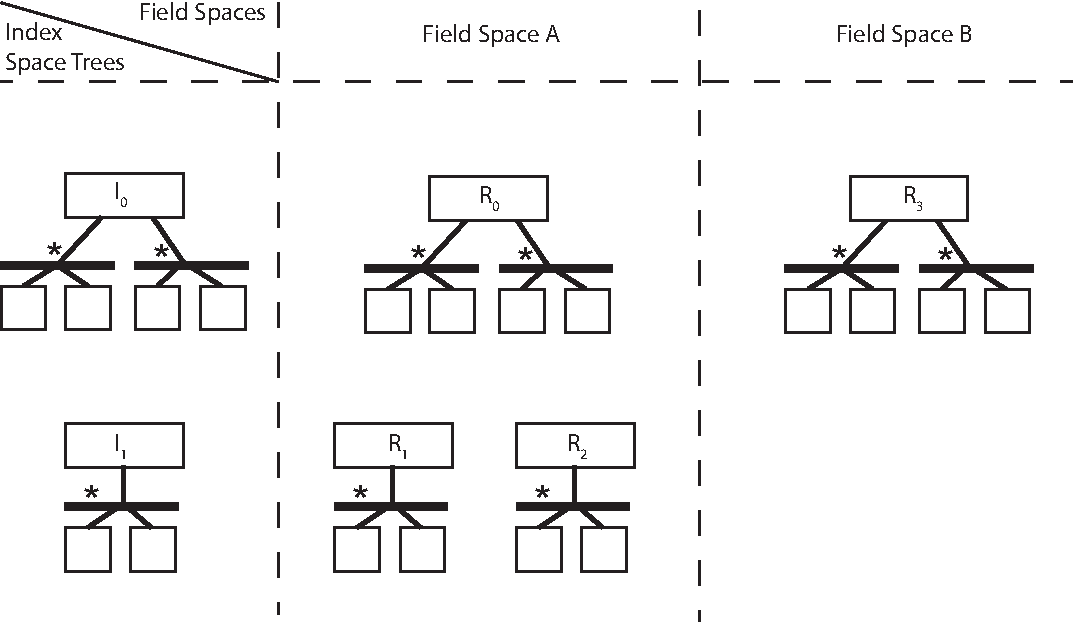
\includegraphics[scale=0.7]{figs/RegionTreeForest}
\caption{Example Relationships Between Index Space Trees, 
Field Spaces, and Logical Region Trees\label{fig:regforest}} 
\end{figure}

Index space trees are eagerly instantiated when
runtime calls are made by the application.  However, 
to save space, logical region trees are lazily
instantiated from index space trees.  When a new
top-level logical region is created, only a node
for that root region is created.  The other nodes
in the region tree are only created when they are
requested as part of a dependence analysis traversal. 
Consequently, on many nodes in the machine, only a subset 
of the full region tree forest is ever instantiated for a 
real Legion application, thereby saving considerable 
space\footnote{To further save memory, The migration of region trees to other nodes 
is also done lazily as we describe in 
Chapter~\ref{chapter:distributed}.}.

Index space tree nodes (and therefore by proxy region
tree nodes) also keep track of two important properties
of their child nodes: disjointness and completeness.  
Disjointness records which children of a node are entirely
independent of each other. Disjointness information
is used by the dependence analysis to determine which
nodes in the region tree must be visited. All logical
regions in sub-trees rooted by a region tree node that
is potentially aliased with another region tree node
along the interference path must be analyzed for 
interference.  In some cases, disjointness information is 
provided by the application, such as when disjoint partitions 
are created, indicating that all pairs of children within a
partition are disjoint. Alternatively, if enabled, the runtime 
can dynamically test whether pairs of children are disjoint 
(e.g. testing  whether two specific logical regions in an 
aliased partition are independent).  In the case of the 
dynamic disjointness tests, the results can be memoized to 
help amortize the cost of performing the (sometimes 
expensive) tests.

The second property recorded by all index space tree
nodes is completeness. A child is considered to be
complete if every row in the index space node is 
contained in at least one child index space. Completeness
will be used to perform several important copy reduction
optimizations described in Chapter~\ref{chapter:physical}.

The disjointness and completeness properties of child 
nodes behave differently under dynamic allocation of
rows in index spaces permitted by the Legion programming
model (see Section~\ref{subsec:indexspace}). The disjointness
of two children is invariant under dynamic allocation.
If a new row is allocated in one child node, then it is
impossible for it to be allocated in the other child
node.  However, completeness of a child node is impacted
by dynamic allocation.  Consider an index space $I$ with
two initially complete index partitions $P_1$ and $P_2$.  
If a new entry is allocated in one of the index sub-spaces 
of $P_1$ it is therefore also allocated in index space $I$.
While $P_1$ is still complete, $P_2$ can no longer be 
considered complete. Therefore, while disjointness information
can be safely memoized under dynamic allocation, completeness
can only be cached and must always be invalidated whenever
dynamic allocation is performed.

\subsection{Epoch Lists}
\label{subsec:epochlists}
The first optimization that we perform is
designed to reduce the number of users that 
must be considered on each node that we 
traverse. The critical insight is that we
don't need to record all dependences that
exist between a task $T$ and earlier tasks
in the stream $S$ if $T$ has transitive
dependences through other tasks in $S$.
While there are many ways that we could detect
transitive dependences, we focus on a subset
of transitive dependences that are easy
to detect: those dependences that exist
through the same field with the same 
logical region. The crucial insight
is that tasks within the same node using
the same fields will form {\em epochs}
of tasks with the same privileges.  For
example, there maybe an epoch of tasks 
performing reductions to a field, followed
by an epoch of tasks that read the field
(note there can also be epochs containing 
multiple tasks with read-write privileges 
by using relaxed coherence modes that 
are discussed in Chapter~\ref{chapter:relaxed}). 
By only storing the most recent epochs of
tasks for each field, we can reduce the
number of tasks that must be considered
when traversing a region tree node.

Figure~\ref{fig:epochlist} shows example
epochs that might be generated from a stream
of tasks (accessing only a single field).
Epoch zero consists of tasks that are all 
accessing the field with read-only privileges. 
The next epoch contains a single read-write
task that records mapping dependences on all
tasks from epoch zero.  Epoch two is a reduction
epoch, while epoch three is again a read-only
epoch. The important observation is that each
operation in an epoch needs to record a dependence
on all operations from the previous epoch.
Therefore at most, two epochs need to be tracked
at a time.

\begin{figure}[t]
\centering
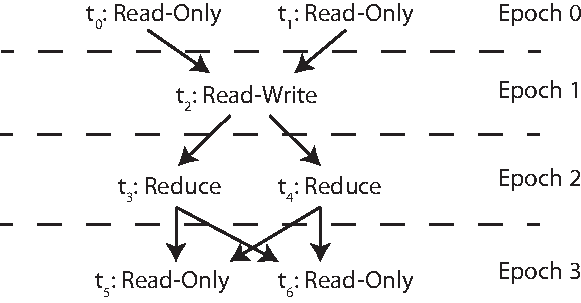
\includegraphics[scale=0.7]{figs/EpochLists}
\caption{Epoch Lists Example\label{fig:epochlist}}
\end{figure}

To track epochs, we create two {\em epoch lists}
that are used to store all the tasks
necessary for performing dependence analysis
in the given node.  The first epoch list stores 
a set of {\em current} epoch users while the 
second list stores the set of {\em previous} 
epoch users. The important observation is that when
performing dependence analysis, only one of
two things will occur: either a user 
will register dependences on all the users 
in the current epoch (for a field), in which
case it will start a new current epoch, or it
will join the current epoch and must therefore
record dependences on all the users 
in the previous epoch list (for a field).
These two epoch lists eliminate the need for 
storing all previous users from the stream of 
tasks not in the two most recent epochs, thereby 
reducing the number of tasks for which we need 
to perform non-interference tests when 
registering a user within a region tree node.

When traversing a given region tree node for
the dependence analysis we need to detect which
of the two scenarios apply to the user 
being analyzed. To detect the first scenario,
we test the region requirement from $T$ being
analyzed against all of the region requirements
in the current epoch list to see if it interferes
with all the users for a specific set of fields.
If the region requirement does interfere with all
users for some set of fields, we say that the
task has {\em dominated} those fields, and should
start a new epoch for those fields. For all the
dominated fields, the users of those fields in the
previous epoch list are filtered out, and the users
from the current epoch list are moved from the 
current epoch list back to the previous epoch 
list. If the region requirement also has non-dominated
fields, then it must also traverse the previous
epoch list to search for interfering region
requirements.  It is important to note
that because we only add region requirements 
at the destination node of the traversal algorithm,
it is possible not to observe any users of
specific fields in the current epoch list.
In these cases, the unobserved fields must
be considered non-dominating fields. The
alternative of considering them dominated 
would result in premature filtering of region
requirements from the previous epoch list.

One important design decision associated with
epoch lists is whether to store previous
users in different lists for every field
or to maintain a single list of tasks and 
filter based on field set disjointness as
part of the traversal. We opted to implement 
the latter, as there can often be hundreds
or thousands of fields that could result
in large list overheads for only a few
users.  Furthermore, most users request multiple
fields that would result in duplicated 
meta-data for the same user over many lists.
Instead we maintain a single current epoch
list and a single previous epoch list and
rely on a fast mechanism for testing for
field set disjointness that we describe
in Section~\ref{subsec:fieldmasks}.

\subsection{Field Masks}
\label{subsec:fieldmasks}
For many Legion applications, including
the combustion simulation S3D discussed
in Chapter~\ref{chapter:s3d}, field spaces
can contain on the order of hundreds to 
thousands of fields. In order to quickly
evaluate the field set disjointness condition
for non-interference, we need an efficient
representation of a set of fields. We use
{\em field masks} that store fields as
bit masks.

Field masks present a very compact way of
representing the potentially large space of 
fields that can be used by region requirements.
It is important to note that we can only 
implement field masks efficiently because of 
the static upper bound on the number of fields
in a field space, which was described as part 
of the Legion programming model in 
Section~\ref{subsec:fieldspace}. Having unbounded
field masks would require dynamic memory allocation
that invalidates many of the important compiler
optimizations that make operations on field
masks fast.

Field masks support all of the common operations
associated with bit masks including conjunction
and disjunction as well as set subtraction. The
three most important operations that are supported
by field masks are conjunction, testing for an 
empty set, and testing for disjointness with 
another field mask. These operations are useful
for detecting the field set disjointness condition
of non-interference and serve as the basis of
region tree traversal algorithms for both logical
state in this chapter as well as physical state
that we discuss in Chapter~\ref{chapter:physical}.
To accelerate these important operations on field
masks we employ a simple optimization technique:
two-level field masks. Two-level field masks
contain a 64-bit summary representation of the 
field mask. A bit set at index $i$ in the summary
mask indicates the presence of at least one set
bit at an index $j$ in the field mask, where
$mod(j,64)==i$. Before actually
testing for conjunction, emptiness, or disjointness
the summary masks for the field masks are tested
first. Since testing the summary masks only involves 
executing a single instruction (on 64-bit architectures), 
it can easily reduce the work associated with important 
field mask operations, especially for field spaces
with large upper bounds on the number of fields.

In the general case, field masks are implemented
using 64-bit unsigned integers.  However, where
possible, our implementation of field masks also
takes advantage of the underlying hardware by
using SSE and AVX vector intrinsics for performing
field mask operations. It is important to note that
these vectorized bit operations do not conflict
with any of the underlying paths for vectorized 
floating point hardware in most processors. Therefore
our field masks do not cause any performance degradation
when floating point units are shared between 
multiple cores within a chip (as is the case on 
same target architectures such as the AMD 
Interlagos architecture).

\subsection{Region Tree States}
\label{subsec:logicalstate}
The next optimization that we perform for the
traversal algorithm adds some additional state
to each node in the region tree to 
reduce the number of sub-trees in the region
tree that must be traversed when checking for
region disjointness in the non-interference test.
In our original version of the algorithm described
in Section~\ref{sec:logtraversal}, we computed
a path from where the parent task $P$ had privileges
to where the region requirement from sub-task $T$
was requesting privileges. In addition to traversing
all of the nodes along this path, we also described
that we needed to check all sub-trees that contain
regions that might not be disjoint from the logical
region in the target region requirement. To avoid
the traversal of many sub-trees, we
add state to every region tree node that records
which sub-trees are {\em open}.  A sub-tree is
open if there exists at least one region requirement
from another sub-task from the stream $S$ that has 
been registered in the sub-tree.  

To further add to our efficiency, we also track the 
fields that are open for different sub-trees, as well 
as the privileges of the open fields.  For example, a 
sub-tree might only be open for one field or a small 
number of fields.  If those fields are disjoint from the 
fields in the region requirement of $T$, then we 
do not need to traverse the sub-tree.  Similarly, 
a sub-tree might be open for a set of fields with 
read-only privileges which indicates that all 
sub-tasks registered in the sub-tree are requesting 
read-only privileges. If the region requirement
from $T$ being analyzed is also requesting read-only
privileges then dependence analysis for the sub-tree 
can be skipped because we know all users are 
non-interfering on privileges.

Care must be taken to maintain the proper state at
each node of the region tree.  Therefore, we perform the 
traversal along the path from where the parent task $P$ 
has privileges to where the region requirement of $T$
is requesting privileges, we {\em open} the appropriate
child nodes and mark which fields are open with
specific privileges. In some cases the correct 
sub-tree might already be open with the same or
a super-set of the privileges necessary (see the
semi-lattice from Figure~\ref{fig:privlattice}).
However, when privileges are different, there are
two possible solutions. First, we could elevate
privileges in the semi-lattice to soundly represent
the set of region requirements in a sub-tree; this
approach is easy to implement, but results in a 
lack of precision. Alternatively,
we could {\em close} all potentially conflicting
sub-trees and then open the sub-tree we intend
to traverse with the precise privileges. In order to 
maintain the fidelity of the dependence analysis, we 
chose to implement the later option.

A close operation on a sub-tree mutates the state 
of the region tree in two ways.  First, a close
operation on a field is the equivalent of dominating
all the users in the current epoch of the node at
the root of the close operation
We therefore siphon all the users for the
field(s) being closed from the previous epoch list
and filter any users from the current epoch list
into the previous epoch list.  We then hoist all
of the tasks in the current epoch lists in the
sub-tree, for the given field(s), up to the previous
epoch list of the node at the root of the sub-tree
being closed. While this reduces the precision of
the tasks for region analysis, it is always sound
as they now appear to be using a region node that 
is a superset of the region node they were
originally using\footnote{Ultimately the loss in 
precision is inconsequential because extra mapping 
dependences need to be computed between users accessing
logical regions in different partitions in order to
correctly perform the pre-mapping traversals described
in Section~\ref{sec:premapping}.}.  Furthermore, this 
loss of precision is minimal since the primary reason
for performing close operations is to open a
different sub-tree whose regions all conflict
the sub-tree being closed (e.g. closing one
partition sub-tree to open another). After the
close operation is complete, the traversal
can continue by opening up the sub-tree of 
the next node in the appropriate mode.

Since close operations effectively mutate the
state of the epoch lists for the fields that
are closed, we record the close operations that
need to be performed between the previous
epoch and the current epoch in a {\em close
list}. It is important that each user added to
the current epoch list of a set of fields also
record dependences on all close operations that
must be performed for those fields. The reason
for this is that these close operations must
be performed prior to mapping any of the region
requirements for a task.
Since multiple tasks in the same epoch are
able to map in parallel, then it is the 
responsibility of the first task that maps
in an epoch to perform the close operations in 
the physical state of the tree. We discuss the 
details of how close operations are performed in the 
physical tree in Chapter~\ref{chapter:physical}.
The close list is also filtered along with the
previous epoch list when one or more fields begins
a new epoch.

\begin{figure}[t]
\centering
\subfloat[State After CNC]{
\label{fig:cktstate_a}
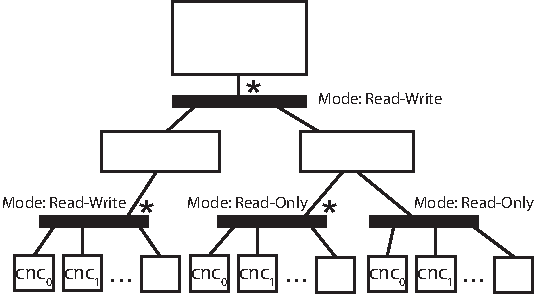
\includegraphics[scale=0.5]{figs/CNC_State}
}
\subfloat[State After DC]{
\label{fig:cktstate_b}
\includegraphics[scale=0.5]{figs/DC_State}
}
\subfloat[State After UV]{
\label{fig:cktstate_c}
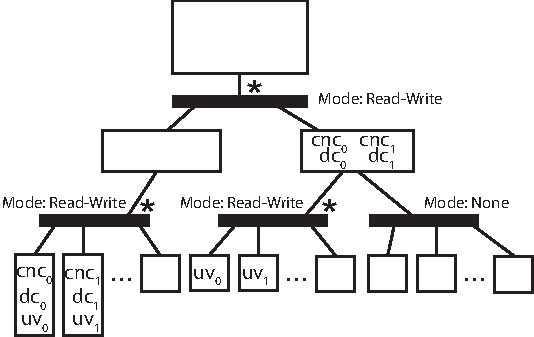
\includegraphics[scale=0.5]{figs/UV_State}
}
\caption{Example Circuit Region Tree States\label{fig:cktstate}}
\end{figure}

Figure~\ref{fig:cktstate} shows the state of the
logical partitions in the node logical region tree
after different sets of task perform their 
dependence analysis. The first set of tasks to
map are the {\tt calculate\_new\_currents} (CNC)
tasks.  In Figure~\ref{fig:cktstate_a}, all of the
CNC tasks have completed their analysis and registered
themselves at the appropriate logical region nodes
based upon their region requirements. In the process
of traversing from the root node, each task has opened
up partitions with the appropriate privileges\footnote{In
practice all nodes (both privileges and logical regions)
must be opened, but we only show the partitions
for simplicity.}. In this example, we show the steady-state
behavior in the middle of the loop, therefore intermediate
partitions are already open with read-write privileges
indicating the existence of modified state from earlier
loop iterations. 

Figure~\ref{fig:cktstate_b} shows the
state of the region tree after the {\tt distribute\_charge}
(DC) tasks have finished their dependence analysis.
Note that all of the CNC tasks in the shared sub-tree have
been moved back to the {\tt all\_shared} logical region
as the result of a close operation necessary to transition
from the partition being open with read-only privileges
to reduction privileges. The {\tt all\_private} sub-region
did not require such a transition as it was already open
with read-write privileges that subsume reduction privileges.
Figure~\ref{fig:cktstate_b} also demonstrates the benefits
of reduction privileges: both the {\tt p\_shr\_nodes} and
{\tt p\_ghost\_nodes} partitions can be open at the same
time with reduction privileges.

Lastly, Figure~\ref{fig:cktstate_c} shows the state of
the region tree after the {\tt update\_voltages} (UV)
tasks have completed their analysis. Another close operation
was necessary to close up the {\tt p\_shr\_nodes} and 
{\tt p\_ghost\_nodes} partitions to transition from 
reduction privileges to the read-write privileges needed
by the UV tasks on the {\tt p\_shr\_nodes} partition.
Each of the UV tasks records a dependence on this close
operation as part of their dependence analysis.

\subsection{Privilege State Transitions}
\label{subsec:statetrans}
Figure~\ref{fig:childstate} shows the state transition
diagram for child nodes based on privileges. For
a given field in a specific state, arcs
show the transition that must occur based on the
privileges being requested by the region requirement
of $T$.  For cases where the state of the privileges
move down or across the privilege semi-lattice, close
operations must first be performed before the next
sub-tree can be opened. One interesting observation 
about this state diagram is that it is very similar
in many ways to the state diagram of directory-based
cache coherence protocols, with the only differences
being that the privilege state diagram has more potential
states (involving reductions), and that the granularity
of logical regions is much larger than individual cache
lines. By operating at a coarser granularity, our Legion
implementation is able to amortize the cost of 
having a more complex state graph and maintain state
for each field of a logical region in software instead 
of in hardware.

% Multiple reductions
% Reduction Optimization
Figure~\ref{fig:childstate} has an interesting property
when it comes to reductions. Note that there exists
an intermediate state called {\em single-reduce}. In
this state, only a single sub-tree is permitted to be
open for a specific kind of reduction. This state acts
as an intermediate state for deferring the decision of 
whether a sub-tree from a node should be opened in 
read-write or reduction mode. The decision is ambiguous
when the first reduction region requirement is registered
in a sub-tree: the runtime cannot be sure whether more 
reductions of the same kind will open other sub-trees, or 
if other operations such as reads or write will be 
performed in the same sub-tree.  If a different kind of
reduction or a read or a write task proceeds down the
same sub-tree, then the state is changed to be in
read-write mode.  However, if a later sub-task 
attempts to open a different sub-tree with the same
reduction mode, then the state is changed to be
in multiple-reduce mode. Deferring the decision about
whether to be in multiple-reduce or read-write mode
for reduction is important because it avoids guessing
by the runtime about the proper way to open the sub-tree,
that could result in unnecessary close operations 
being performed.

\begin{figure}
\begin{tikzpicture}[->,>=stealth',shorten >=1pt,auto,node distance=4cm,thick]

\node[initial,state,initial text=] (A) {Closed};
\node[state] (B) [below=3cm of A] {Read-Only};
\node[state] (C) [above right=1cm and 4.5cm of A] {Multiple-Reduce};
\node[state] (D) [below=2cm of C] {Single-Reduce};
\node[state] (E) [below=2cm of D] {Read-Write};

% Arrows from close
\path[->,anchor=east] (A) edge [bend right] node {read} (B);
\path[->,anchor=north] (A) edge [bend left] node {reduce} (D);
\path[->,anchor=east] (A) edge [bend right,pos=0.75] node {write} (E);

% Arrows from read-only
\path[->,anchor=west] (B) edge [bend right] node {close} (A);
\path[->,anchor=north] (B) edge [bend right] node {write} (E);
\path[->,anchor=east] (B) edge [bend left,right,pos=0.25] node {reduce} (D);
\path[->,anchor=east] (B) edge [loop below] node {read} (B);

% Arrows from read-write
\path[->,anchor=west] (E) edge [bend right,pos=0.15] node {close} (A);
\path[->,anchor=east] (E) edge [loop right] node {read,write,reduce} (E);

% Arrows for single-reduce
\path[->,anchor=east] (D) edge [bend left,right] node[align=center] {read,\\reduce (diff. op. or\\diff. child),\\write} (E);
\path[->,anchor=east] (D) edge [bend right,right] node[align=center] {reduce (same op. and\\diff child)} (C);
\path[->,anchor=east] (D) edge [loop right,right] node[align=center] {reduce (same op. and\\same child)} (D);
\path[->,anchor=north] (D) edge [bend left,pos=0.3] node {close} (A);

% Arrows for multi-reduce
\path[->,anchor=south] (C) edge [bend right,below] node {close} (A);
\path[->,anchor=north] (C) edge [loop right] node {reduce (same op.)} (C);

\end{tikzpicture}
\caption{Open Child Privilege State Diagram\label{fig:childstate}}
\end{figure}

\subsection{Logical Contexts}
\label{subsec:logicalctx}
The final optimization that we perform on 
region trees is designed to reduce the memory
usage required for storing state associated
with region trees. Recall from 
Section~\ref{subsec:logicalshape} that region
tree data structures are de-duplicated across
runtime instances. Since there may be many
tasks executing simultaneously within a runtime
instance, all of these tasks will be generating
different streams of sub-tasks.  We therefore
need a mechanism for differentiating the state
that must be stored in the region tree forest
from different streams of tasks.

This is achieved by differentiating
different streams of sub-tasks as {\em logical
contexts}.  On every node in the region tree
forest there exists an array of {\em logical
state} objects that store the necessary meta-data
for supporting the logical region tree traversal
algorithms described in this chapter (e.g. 
epoch lists, close lists, open children). The
array of logical state objects is indexed by a
logical context ID. Before a parent task $P$
begins to execute, it requests a logical context
ID from the runtime.  When $P$ executes,
it generates a stream of sub-tasks all of which
are analyzed within the logical context allocated
to the parent, meaning they use the parent's
logical context ID to index into the logical
state arrays on the region tree nodes when
performing their dependence analysis.

In order to ensure correctness of Legion programs,
before executing, each task is allocated a logical 
context by the runtime instance. This is necessary 
since any task can launch arbitrary sub-tasks.  
However, logical contexts can be an expensive 
resource to allocate because of the implied memory
usage required on all instantiated nodes of a region
tree. To reduce context usage, Legion programmers
can indicate that certain task variants are 
actually leaf task variants 
(see Section~\ref{subsec:qualifiers}).  Leaf task
variants are guaranteed not to perform any sub-task
or other operation launches.
The knowledge that no sub-tasks will be launched
by an executing task is sufficient to allow the
runtime to elide the allocation of a context to 
the executing task, thereby reducing both context 
and memory usage.

\section{Dynamic Dependence Graph}
\label{sec:mapdepgraph}
The result of the dependence analysis stage
is a {\em dynamic dependence graph} for a
given stream of operations generated by a parent 
task. The dynamic dependence graph is a directed 
acyclic graph where nodes represent operations 
(e.g. sub-tasks, inline mappings, explicit region
copies) and edges represent dependences that
result from interfering region requirements.
It is impossible for there to exist cycles in
this graph as the dependence analysis stage
is performed serially for all sub-tasks
within the stream $S$ generated by parent 
task $P$. While there are no
cycles within the dynamic dependence graph,
there can be multiple edges between nodes as
sub-tasks may have multiple interfering 
region requirements. Exactly one dynamic
dependence graph is computed for the execution
of each parent task. While the entire graph
needs to be computed, we describe how the
entire dynamic dependence graph does not
need to persist throughout the lifetime of
the parent task $P$.

Figure~\ref{fig:s3ddg} shows an example dynamic
dependence graph from the S3D application 
described in detail in Chapter~\ref{chapter:s3d}.
Boxes represent operations that are performed as
part of the computation while edges represent
computed dependences between operations as a
result of the logical dependence analysis.
Edges primarily point from left to right.
The vertical span of the graph is therefore
indicative of the amount of task-level parallelism
available in S3D. It is important to realize
that this graph was generated from a fraction of
a time step in S3D for the smallest chemical
mechanism possible. Production S3D runs generate
graphs that would consume many pages if 
depicted here.

\begin{figure}[ht!]
\centering
\includegraphics[scale=0.06]{figs/s3d_h2_smart_mapper}
\caption{Example Dynamic Dependence Graph from S3D\label{fig:s3ddg}}
\end{figure}

The directed edges indicating interference
between sub-tasks serve a dual purpose. First,
dependences between sub-tasks are used to determine
when it is safe for a sub-task to progress to
the mapping stage of the pipeline.  A task is
only permitted to progress to the mapping stage
once all of the sub-tasks on which it has a
dependence have finished the mapping stage of
the pipeline. Under these circumstances, we
refer to the edges as {\em mapping dependences}.
By requiring all mapping dependences be
satisfied for a sub-task before it can map,
we ensure that it will properly compute any
dependences (either true or anti-dependences)
as part of its physical analysis (see
Chapter~\ref{chapter:physical}). To know when
mapping dependences have been satisfied, sub-tasks
register themselves with the source sub-tasks
of all their dependence edges. If the source
sub-task has yet to map, it will accept the
registration, otherwise it will indicate that
it has already finished the mapping stage
of the pipeline and indicate that no mapping
dependence is necessary.
Each sub-task records how many successful
registrations it makes; this is the number
of other sub-tasks that it must wait to
complete the mapping stage before it can progress
to the mapping stage. When a task finishes
the mapping stage, it notifies all its
registered waiters to indicate that it has
finished mapping. If any of the waiters no
longer have any outstanding registrations, then
they are placed on the {\em ready queue} of 
tasks that are ready to map, and the mapper
is queried to choose which tasks in the
ready queue should be mapped next (see 
Section~\ref{sec:mapbasic} for more details
on mapper queries and the ready queue).

The second purpose of the edges in the
dynamic dependence graph are to act as
{\em commit edges}. Edges which represent
true data dependences (those on which the
privilege of the source is a reduction or 
a write, and the privilege of the 
destination is either read-only or read-write)
and for which the destination logical region
is at least as large as the source logical
region are considered commit edges.  Commit
edges help to govern the reclamation of the
dynamic dependence graph so that the entire
graph need not persist throughout
the duration of the execution of the parent 
task. Long running parent tasks can generate 
hundreds or even thousands of sub-tasks and 
operations, resulting in very large dynamic 
dependence graphs.  As tasks finish, commit edges 
govern the parts of the dynamic dependence
graph that can be reclaimed.

The direction of commit edges is the 
opposite of the direction for dependences
in the dynamic dependence graph. Every
node $N$ in the dynamic dependence graph 
registers itself with all of the other
nodes that are sources on commit edges
that point to $N$. As tasks commit, they
notify all tasks that have registered
commit dependences on them.  If at any
point all of the commit edges pointing
at a node have been satisfied then the
node can be safely reclaimed.  The 
intuition is that once all the commit
edges have been satisfied, then there
are no later tasks in the stream of 
sub-tasks $S$ that can trigger a 
roll-back that might require a
re-execution of the task at node $N$.
There are two other ways in which tasks
can pass the commit stage that allows
them to be reclaimed, both of  which are discussed
in Chapters~\ref{chapter:mapping} and
\ref{chapter:resilience} respectively.

Due to the number of places in both the
region tree forest and the dynamic
dependence graph that contain references 
to objects that represent sub-task and
other operations, it is expensive to 
go through all these data structures 
and prune out references. Instead, we
borrow an idea from \cite{Realm14} and
recycle the objects that represent
sub-tasks and other operations. We 
assign each use of these objects a 
{\em generation} that identifies a
specific operation that the task is
using.  We then update all references
to these objects to include the generation.
All methods on the object (e.g. for 
performing registration) require that
the generation be passed as well. If
the generation is older than the current
generation, then the method will return
that the version of the operation 
being referenced has already committed.
Once a task has committed, it increments
its generation, and then adds itself
back to the pool of available objects
managed by the runtime to be recycled.

\section{Memoizing Logical Dependence Traces}
\label{sec:tracing}

One very important optimization that the
dependence analysis stage supports is the ability
to capture {\em traces} of task executions.
Capturing traces of sub-tasks is inspired by
and has a direct analogy to a common feature
in hardware out-of-order processors: trace
caches. The idea behind capturing traces of
execution is that the dependence analysis
stage is the only inherently sequential 
computation in the Legion task pipeline. All
other stages permit multiple tasks or operations
to be processed in parallel. The sequential
nature of this stage means that it can be
very expensive to do for large numbers of
tasks.  By capturing traces of a subset
of operations in a stream, we can memoize
the dependence analysis results and replay
them later when the trace is encountered again.

The motivation for incorporating trace capture
as an important optimization is that many 
Legion applications employ 
large loops of repetitive task execution. For
example, most scientific simulations execute
for a large number of time steps, executing
either the same or similar sets of tasks
for each time step. Similarly, iterative
solvers execute the same set of tasks until
they converge. Owing to the multitude of 
Legion applications that share this structure,
we deemed it prudent to include tracing as
an optimization.

Unlike traditional hardware trace caches that 
are invisible to the application, the Legion
programming model requires applications to 
explicitly indicate the beginning and end of
a trace with a runtime call. Both the start
and end runtime call
take a trace ID parameter for identifying
the trace. The first time a dynamic trace ID
is encountered within a context, the runtime 
initializes an object for capturing the trace. 
Each sub-task or other operation that is 
launched during the trace is recorded. All 
dependences in the dynamic dependence graph 
between operations in the trace are also 
recorded. Dependences between an operation 
inside the trace and a second 
operation outside of the trace are not 
recorded. As we will see, we rely on a second 
mechanism to handle these dependences when 
the trace is re-executed. It is important to 
note that we can eagerly prune dependences
for tasks that have already finished executing
when capturing a trace. Even through some operations
in a trace may have already committed, which
commonly occurs in larger traces, we still must
record the dependences since there is no
guarantee that the same scenario will occur
when the trace is replayed. Once the trace 
capture is complete, the trace is frozen and 
can be re-used. Trace objects only exist within
the context of a parent task and are automatically 
reclaimed when the parent task completes.

After a trace has been captured, the next
time the trace is encountered, the Legion
runtime can automatically replay the results
of the dependence analysis stage instead
of having to recompute the dependences.
In order to avoid missing dependences between
operations within the trace and operations
that come before and after the trace, the
runtime inserts a mapping fence (see 
Section~\ref{subsec:fences}) both before 
the trace begins and after the trace ends.
These fences ensure that any missing 
dependences across the trace boundary are
included.  While these fences do add additional
dependences to the dynamic dependence graph
which may constrain execution, the assumption
is that the size of the trace will be 
sufficiently large to amortize the additional
cost of the mapping fences.

Another important requirement of the tracing
feature is that the re-execution of the trace
executes an identical stream of operations
to the one that was captured. The onus is
currently on the user to guarantee this 
property, and any failure to maintain this
invariant will result in a runtime error. In the 
future, we hope that additional logic can be 
added to both the Legion compiler and runtime to
automatically add support for tracing.  It
may be possible for the Legion runtime to
recognize long streams of isomorphic tasks
that are constantly replayed and should
therefore be traced.  Furthermore, it should
be possible for the Legion compiler to 
recognize loops in Legion tasks that generate
the same stream of sub-tasks with no
control statements and insert the proper 
tracing calls.

